%%%%%%%%%%%%%%%%%%%%%%%%%%%%%%%%%%%%%%%%%
% The Legrand Orange Book
% LaTeX Template
% Version 2.4 (26/09/2018)
%
% This template was downloaded from:
% http://www.LaTeXTemplates.com
%
% Original author:
% Mathias Legrand (legrand.mathias@gmail.com) with modifications by:
% Vel (vel@latextemplates.com)
%
% License:
% CC BY-NC-SA 3.0 (http://creativecommons.org/licenses/by-nc-sa/3.0/)
%
% Compiling this template:
% This template uses biber for its bibliography and makeindex for its index.
% When you first open the template, compile it from the command line with the 
% commands below to make sure your LaTeX distribution is configured correctly:
%
% 1) pdflatex main
% 2) makeindex main.idx -s StyleInd.ist
% 3) biber main
% 4) pdflatex main x 2
%
% After this, when you wish to update the bibliography/index use the appropriate
% command above and make sure to compile with pdflatex several times 
% afterwards to propagate your changes to the document.
%
% This template also uses a number of packages which may need to be
% updated to the newest versions for the template to compile. It is strongly
% recommended you update your LaTeX distribution if you have any
% compilation errors.
%
% Important note:
% Chapter heading images should have a 2:1 width:height ratio,
% e.g. 920px width and 460px height.
%
%%%%%%%%%%%%%%%%%%%%%%%%%%%%%%%%%%%%%%%%%

%----------------------------------------------------------------------------------------
%	PACKAGES AND OTHER DOCUMENT CONFIGURATIONS
%----------------------------------------------------------------------------------------

\documentclass[11pt,fleqn]{book} % Default font size and left-justified equations

%%%%%%%%%%%%%%%%%%%%%%%%%%%%%%%%%%%%%%%%%
% The Legrand Orange Book
% Structural Definitions File
% Version 2.1 (26/09/2018)
%
% Original author:
% Mathias Legrand (legrand.mathias@gmail.com) with modifications by:
% Vel (vel@latextemplates.com)
% 
% This file was downloaded from:
% http://www.LaTeXTemplates.com
%
% License:
% CC BY-NC-SA 3.0 (http://creativecommons.org/licenses/by-nc-sa/3.0/)
%
%%%%%%%%%%%%%%%%%%%%%%%%%%%%%%%%%%%%%%%%%

%----------------------------------------------------------------------------------------
%	VARIOUS REQUIRED PACKAGES AND CONFIGURATIONS
%----------------------------------------------------------------------------------------

\usepackage{graphicx} % Required for including pictures
%\graphicspath{{Pictures/}} % Specifies the directory where pictures are stored

\usepackage{lipsum} % Inserts dummy text

\usepackage{tikz} % Required for drawing custom shapes

\usepackage[spanish]{babel} % English language/hyphenation

\usepackage{enumitem} % Customize lists
\setlist{nolistsep} % Reduce spacing between bullet points and numbered lists

\usepackage{booktabs} % Required for nicer horizontal rules in tables

\usepackage{xcolor} % Required for specifying colors by name
\definecolor{ocre}{RGB}{0,32,96}% Define the orange color used for highlighting throughout the book

%----------------------------------------------------------------------------------------
%	MARGINS
%----------------------------------------------------------------------------------------

\usepackage{geometry} % Required for adjusting page dimensions and margins

\geometry{
	paper=a4paper, % Paper size, change to letterpaper for US letter size
	top=3cm, % Top margin
	bottom=3cm, % Bottom margin
	left=3cm, % Left margin
	right=3cm, % Right margin
	headheight=14pt, % Header height
	footskip=1.4cm, % Space from the bottom margin to the baseline of the footer
	headsep=10pt, % Space from the top margin to the baseline of the header
	%showframe, % Uncomment to show how the type block is set on the page
}

%----------------------------------------------------------------------------------------
%	FONTS
%----------------------------------------------------------------------------------------

\usepackage{avant} % Use the Avantgarde font for headings
%\usepackage{times} % Use the Times font for headings
\usepackage{mathptmx} % Use the Adobe Times Roman as the default text font together with math symbols from the Sym­bol, Chancery and Com­puter Modern fonts

\usepackage{microtype} % Slightly tweak font spacing for aesthetics
\usepackage[utf8]{inputenc} % Required for including letters with accents
\usepackage[T1]{fontenc} % Use 8-bit encoding that has 256 glyphs

%----------------------------------------------------------------------------------------
%	BIBLIOGRAPHY AND INDEX
%----------------------------------------------------------------------------------------

\usepackage[style=numeric,citestyle=numeric,sorting=nyt,sortcites=true,autopunct=true,babel=hyphen,hyperref=true,abbreviate=false,backref=true,backend=biber]{biblatex}
\addbibresource{bibliography.bib} % BibTeX bibliography file
\defbibheading{bibempty}{}

\usepackage{calc} % For simpler calculation - used for spacing the index letter headings correctly
\usepackage{makeidx} % Required to make an index
\makeindex % Tells LaTeX to create the files required for indexing

%----------------------------------------------------------------------------------------
%	MAIN TABLE OF CONTENTS
%----------------------------------------------------------------------------------------

\usepackage{titletoc} % Required for manipulating the table of contents

\contentsmargin{0cm} % Removes the default margin

% Part text styling (this is mostly taken care of in the PART HEADINGS section of this file)
\titlecontents{part}
	[0cm] % Left indentation
	{\addvspace{20pt}\bfseries} % Spacing and font options for parts
	{}
	{}
	{}

% Chapter text styling
\titlecontents{chapter}
	[1.25cm] % Left indentation
	{\addvspace{12pt}\large\sffamily\bfseries} % Spacing and font options for chapters
	{\color{blue!60}\contentslabel[\Large\thecontentslabel]{1.25cm}\color{blue}} % Formatting of numbered sections of this type
	{\color{blue}} % Formatting of numberless sections of this type
	{\color{blue!60}\normalsize\;\titlerule*[.5pc]{.}\;\thecontentspage} % Formatting of the filler to the right of the heading and the page number

% Section text styling
\titlecontents{section}
	[1.25cm] % Left indentation
	{\addvspace{3pt}\sffamily\bfseries} % Spacing and font options for sections
	{\contentslabel[\thecontentslabel]{1.25cm}} % Formatting of numbered sections of this type
	{} % Formatting of numberless sections of this type
	{\hfill\color{black}\thecontentspage} % Formatting of the filler to the right of the heading and the page number

% Subsection text styling
\titlecontents{subsection}
	[1.25cm] % Left indentation
	{\addvspace{1pt}\sffamily\small} % Spacing and font options for subsections
	{\contentslabel[\thecontentslabel]{1.25cm}} % Formatting of numbered sections of this type
	{} % Formatting of numberless sections of this type
	{\ \titlerule*[.5pc]{.}\;\thecontentspage} % Formatting of the filler to the right of the heading and the page number

% Figure text styling
\titlecontents{figure}
	[1.25cm] % Left indentation
	{\addvspace{1pt}\sffamily\small} % Spacing and font options for figures
	{\thecontentslabel\hspace*{1em}} % Formatting of numbered sections of this type
	{} % Formatting of numberless sections of this type
	{\ \titlerule*[.5pc]{.}\;\thecontentspage} % Formatting of the filler to the right of the heading and the page number

% Table text styling
\titlecontents{table}
	[1.25cm] % Left indentation
	{\addvspace{1pt}\sffamily\small} % Spacing and font options for tables
	{\thecontentslabel\hspace*{1em}} % Formatting of numbered sections of this type
	{} % Formatting of numberless sections of this type
	{\ \titlerule*[.5pc]{.}\;\thecontentspage} % Formatting of the filler to the right of the heading and the page number

%----------------------------------------------------------------------------------------
%	MINI TABLE OF CONTENTS IN PART HEADS
%----------------------------------------------------------------------------------------

% Chapter text styling
\titlecontents{lchapter}
	[0em] % Left indentation
	{\addvspace{15pt}\large\sffamily\bfseries} % Spacing and font options for chapters
	{\color{blue}\contentslabel[\Large\thecontentslabel]{1.25cm}\color{blue}} % Chapter number
	{}  
	{\color{blue}\normalsize\sffamily\bfseries\;\titlerule*[.5pc]{.}\;\thecontentspage} % Page number

% Section text styling
\titlecontents{lsection}
	[0em] % Left indentation
	{\sffamily\small} % Spacing and font options for sections
	{\contentslabel[\thecontentslabel]{1.25cm}} % Section number
	{}
	{}

% Subsection text styling (note these aren't shown by default, display them by searchings this file for tocdepth and reading the commented text)
\titlecontents{lsubsection}
	[.5em] % Left indentation
	{\sffamily\footnotesize} % Spacing and font options for subsections
	{\contentslabel[\thecontentslabel]{1.25cm}}
	{}
	{}

%----------------------------------------------------------------------------------------
%	HEADERS AND FOOTERS
%----------------------------------------------------------------------------------------

\usepackage{fancyhdr} % Required for header and footer configuration

\pagestyle{fancy} % Enable the custom headers and footers

\renewcommand{\chaptermark}[1]{\markboth{\sffamily\normalsize\bfseries\chaptername\ \thechapter.\ #1}{}} % Styling for the current chapter in the header
\renewcommand{\sectionmark}[1]{\markright{\sffamily\normalsize\thesection\hspace{5pt}#1}{}} % Styling for the current section in the header

\fancyhf{} % Clear default headers and footers
\fancyhead[LE,RO]{\sffamily\normalsize\thepage} % Styling for the page number in the header
\fancyhead[LO]{\rightmark} % Print the nearest section name on the left side of odd pages
\fancyhead[RE]{\leftmark} % Print the current chapter name on the right side of even pages
%\fancyfoot[C]{\thepage} % Uncomment to include a footer

\renewcommand{\headrulewidth}{0.5pt} % Thickness of the rule under the header

\fancypagestyle{plain}{% Style for when a plain pagestyle is specified
	\fancyhead{}\renewcommand{\headrulewidth}{0pt}%
}

% Removes the header from odd empty pages at the end of chapters
\makeatletter
\renewcommand{\cleardoublepage}{
\clearpage\ifodd\c@page\else
\hbox{}
\vspace*{\fill}
\thispagestyle{empty}
\newpage
\fi}

%----------------------------------------------------------------------------------------
%	THEOREM STYLES
%----------------------------------------------------------------------------------------

\usepackage{amsmath,amsfonts,amssymb,amsthm} % For math equations, theorems, symbols, etc

\newcommand{\intoo}[2]{\mathopen{]}#1\,;#2\mathclose{[}}
\newcommand{\ud}{\mathop{\mathrm{{}d}}\mathopen{}}
\newcommand{\intff}[2]{\mathopen{[}#1\,;#2\mathclose{]}}
\renewcommand{\qedsymbol}{$\blacksquare$}
\newtheorem{notation}{Nota}[chapter]

% Boxed/framed environments
\newtheoremstyle{bluenumbox}% Theorem style name
{0pt}% Space above
{0pt}% Space below
{\normalfont}% Body font
{}% Indent amount
{\small\bf\sffamily\color{blue}}% Theorem head font
{\;}% Punctuation after theorem head
{0.25em}% Space after theorem head
{\small\sffamily\color{blue}\thmname{#1}\nobreakspace\thmnumber{\@ifnotempty{#1}{}\@upn{#2}}% Theorem text (e.g. Theorem 2.1)
\thmnote{\nobreakspace\the\thm@notefont\sffamily\bfseries\color{black}---\nobreakspace#3.}} % Optional theorem note

\newtheoremstyle{blacknumex}% Theorem style name
{5pt}% Space above
{5pt}% Space below
{\normalfont}% Body font
{} % Indent amount
{\small\bf\sffamily}% Theorem head font
{\;}% Punctuation after theorem head
{0.25em}% Space after theorem head
{\small\sffamily{\tiny\ensuremath{\blacksquare}}\nobreakspace\thmname{#1}\nobreakspace\thmnumber{\@ifnotempty{#1}{}\@upn{#2}}% Theorem text (e.g. Theorem 2.1)
\thmnote{\nobreakspace\the\thm@notefont\sffamily\bfseries---\nobreakspace#3.}}% Optional theorem note

\newtheoremstyle{blacknumbox} % Theorem style name
{0pt}% Space above
{0pt}% Space below
{\normalfont}% Body font
{}% Indent amount
{\small\bf\sffamily}% Theorem head font
{\;}% Punctuation after theorem head
{0.25em}% Space after theorem head
{\small\sffamily\thmname{#1}\nobreakspace\thmnumber{\@ifnotempty{#1}{}\@upn{#2}}% Theorem text (e.g. Theorem 2.1)
\thmnote{\nobreakspace\the\thm@notefont\sffamily\bfseries---\nobreakspace#3.}}% Optional theorem note

% Non-boxed/non-framed environments
\newtheoremstyle{bluenum}% Theorem style name
{5pt}% Space above
{5pt}% Space below
{\normalfont}% Body font
{}% Indent amount
{\small\bf\sffamily\color{blue}}% Theorem head font
{\;}% Punctuation after theorem head
{0.25em}% Space after theorem head
{\small\sffamily\color{blue}\thmname{#1}\nobreakspace\thmnumber{\@ifnotempty{#1}{}\@upn{#2}}% Theorem text (e.g. Theorem 2.1)
\thmnote{\nobreakspace\the\thm@notefont\sffamily\bfseries\color{black}---\nobreakspace#3.}} % Optional theorem note
\makeatother

% Defines the theorem text style for each type of theorem to one of the three styles above
\newcounter{dummy} 
\numberwithin{dummy}{section}
\theoremstyle{bluenumbox}
\newtheorem{theoremeT}[dummy]{Teorema}
\newtheorem{problem}{Problema}[chapter]
\newtheorem{exerciseT}{Ejercicio}[chapter]
\theoremstyle{blacknumex}
\newtheorem{exampleT}{Ejemplo}[chapter]
\theoremstyle{blacknumbox}
\newtheorem{vocabulary}{Vocabulario}[chapter]
\newtheorem{definitionT}{Definición}[section]
\newtheorem{corollaryT}[dummy]{Corolario}
\theoremstyle{bluenum}
\newtheorem{proposition}[dummy]{Proposición}

%----------------------------------------------------------------------------------------
%	DEFINITION OF COLORED BOXES
%----------------------------------------------------------------------------------------

\RequirePackage[framemethod=default]{mdframed} % Required for creating the theorem, definition, exercise and corollary boxes

% Theorem box
\newmdenv[skipabove=7pt,
skipbelow=7pt,
backgroundcolor=black!5,
linecolor=purple,
innerleftmargin=5pt,
innerrightmargin=5pt,
innertopmargin=5pt,
leftmargin=0cm,
rightmargin=0cm,
innerbottommargin=5pt]{tBox}

% Exercise box	  
\newmdenv[skipabove=7pt,
skipbelow=7pt,
rightline=false,
leftline=true,
topline=false,
bottomline=false,
backgroundcolor=blue!10,
linecolor=blue,
innerleftmargin=5pt,
innerrightmargin=5pt,
innertopmargin=5pt,
innerbottommargin=5pt,
leftmargin=0cm,
rightmargin=0cm,
linewidth=4pt]{eBox}	

% Definition box
\newmdenv[skipabove=7pt,
skipbelow=7pt,
rightline=false,
leftline=true,
topline=false,
bottomline=false,
linecolor=blue,
innerleftmargin=5pt,
innerrightmargin=5pt,
innertopmargin=0pt,
leftmargin=0cm,
rightmargin=0cm,
linewidth=4pt,
innerbottommargin=0pt]{dBox}	

% Corollary box
\newmdenv[skipabove=7pt,
skipbelow=7pt,
rightline=false,
leftline=true,
topline=false,
bottomline=false,
linecolor=gray,
backgroundcolor=black!5,
innerleftmargin=5pt,
innerrightmargin=5pt,
innertopmargin=5pt,
leftmargin=0cm,
rightmargin=0cm,
linewidth=4pt,
innerbottommargin=5pt]{cBox}

% Creates an environment for each type of theorem and assigns it a theorem text style from the "Theorem Styles" section above and a colored box from above
\newenvironment{theorem}{\begin{tBox}\begin{theoremeT}}{\end{theoremeT}\end{tBox}}
\newenvironment{exercise}{\begin{eBox}\begin{exerciseT}}{\hfill{\color{blue}\tiny\ensuremath{\blacksquare}}\end{exerciseT}\end{eBox}}				  
\newenvironment{definition}{\begin{dBox}\begin{definitionT}}{\end{definitionT}\end{dBox}}	
\newenvironment{example}{\begin{exampleT}}{\hfill{\tiny\ensuremath{\blacksquare}}\end{exampleT}}		
\newenvironment{corollary}{\begin{cBox}\begin{corollaryT}}{\end{corollaryT}\end{cBox}}	

%----------------------------------------------------------------------------------------
%	REMARK ENVIRONMENT
%----------------------------------------------------------------------------------------

\newenvironment{remark}{\par\vspace{10pt}\small % Vertical white space above the remark and smaller font size
\begin{list}{}{
\leftmargin=35pt % Indentation on the left
\rightmargin=25pt}\item\ignorespaces % Indentation on the right
\makebox[-2.5pt]{\begin{tikzpicture}[overlay]
\node[draw=blue!60,line width=1pt,circle,fill=blue!25,font=\sffamily\bfseries,inner sep=2pt,outer sep=0pt] at (-15pt,0pt){\textcolor{blue}{R}};\end{tikzpicture}} % Orange R in a circle
\advance\baselineskip -1pt}{\end{list}\vskip5pt} % Tighter line spacing and white space after remark

%----------------------------------------------------------------------------------------
%	SECTION NUMBERING IN THE MARGIN
%----------------------------------------------------------------------------------------

\makeatletter
\renewcommand{\@seccntformat}[1]{\llap{\textcolor{blue}{\csname the#1\endcsname}\hspace{1em}}}                    
\renewcommand{\section}{\@startsection{section}{1}{\z@}
{-4ex \@plus -1ex \@minus -.4ex}
{1ex \@plus.2ex }
{\normalfont\large\sffamily\bfseries}}
\renewcommand{\subsection}{\@startsection {subsection}{2}{\z@}
{-3ex \@plus -0.1ex \@minus -.4ex}
{0.5ex \@plus.2ex }
{\normalfont\sffamily\bfseries}}
\renewcommand{\subsubsection}{\@startsection {subsubsection}{3}{\z@}
{-2ex \@plus -0.1ex \@minus -.2ex}
{.2ex \@plus.2ex }
{\normalfont\small\sffamily\bfseries}}                        
\renewcommand\paragraph{\@startsection{paragraph}{4}{\z@}
{-2ex \@plus-.2ex \@minus .2ex}
{.1ex}
{\normalfont\small\sffamily\bfseries}}

%----------------------------------------------------------------------------------------
%	PART HEADINGS
%----------------------------------------------------------------------------------------

% Numbered part in the table of contents
\newcommand{\@mypartnumtocformat}[2]{%
	\setlength\fboxsep{0pt}%
	\noindent\colorbox{blue!20}{\strut\parbox[c][.7cm]{\ecart}{\color{blue!70}\Large\sffamily\bfseries\centering#1}}\hskip\esp\colorbox{blue!40}{\strut\parbox[c][.7cm]{\linewidth-\ecart-\esp}{\Large\sffamily\centering#2}}%
}

% Unnumbered part in the table of contents
\newcommand{\@myparttocformat}[1]{%
	\setlength\fboxsep{0pt}%
	\noindent\colorbox{blue!40}{\strut\parbox[c][.7cm]{\linewidth}{\Large\sffamily\centering#1}}%
}

\newlength\esp
\setlength\esp{4pt}
\newlength\ecart
\setlength\ecart{1.2cm-\esp}
\newcommand{\thepartimage}{}%
\newcommand{\partimage}[1]{\renewcommand{\thepartimage}{#1}}%
\def\@part[#1]#2{%
\ifnum \c@secnumdepth >-2\relax%
\refstepcounter{part}%
\addcontentsline{toc}{part}{\texorpdfstring{\protect\@mypartnumtocformat{\thepart}{#1}}{\partname~\thepart\ ---\ #1}}
\else%
\addcontentsline{toc}{part}{\texorpdfstring{\protect\@myparttocformat{#1}}{#1}}%
\fi%
\startcontents%
\markboth{}{}%
{\thispagestyle{empty}%
\begin{tikzpicture}[remember picture,overlay]%
\node at (current page.north west){\begin{tikzpicture}[remember picture,overlay]%	
\fill[blue!20](0cm,0cm) rectangle (\paperwidth,-\paperheight);
\node[anchor=north] at (4cm,-3.25cm){\color{blue!40}\fontsize{220}{100}\sffamily\bfseries\thepart}; 
\node[anchor=south east] at (\paperwidth-1cm,-\paperheight+1cm){\parbox[t][][t]{8.5cm}{
\printcontents{l}{0}{\setcounter{tocdepth}{1}}% The depth to which the Part mini table of contents displays headings; 0 for chapters only, 1 for chapters and sections and 2 for chapters, sections and subsections
}};
\node[anchor=north east] at (\paperwidth-1.5cm,-3.25cm){\parbox[t][][t]{15cm}{\strut\raggedleft\color{white}\fontsize{30}{30}\sffamily\bfseries#2}};
\end{tikzpicture}};
\end{tikzpicture}}%
\@endpart}
\def\@spart#1{%
\startcontents%
\phantomsection
{\thispagestyle{empty}%
\begin{tikzpicture}[remember picture,overlay]%
\node at (current page.north west){\begin{tikzpicture}[remember picture,overlay]%	
\fill[blue!20](0cm,0cm) rectangle (\paperwidth,-\paperheight);
\node[anchor=north east] at (\paperwidth-1.5cm,-3.25cm){\parbox[t][][t]{15cm}{\strut\raggedleft\color{white}\fontsize{30}{30}\sffamily\bfseries#1}};
\end{tikzpicture}};
\end{tikzpicture}}
\addcontentsline{toc}{part}{\texorpdfstring{%
\setlength\fboxsep{0pt}%
\noindent\protect\colorbox{blue!40}{\strut\protect\parbox[c][.7cm]{\linewidth}{\Large\sffamily\protect\centering #1\quad\mbox{}}}}{#1}}%
\@endpart}
\def\@endpart{\vfil\newpage
\if@twoside
\if@openright
\null
\thispagestyle{empty}%
\newpage
\fi
\fi
\if@tempswa
\twocolumn
\fi}

%----------------------------------------------------------------------------------------
%	CHAPTER HEADINGS
%----------------------------------------------------------------------------------------

% A switch to conditionally include a picture, implemented by Christian Hupfer
\newif\ifusechapterimage
\usechapterimagetrue
\newcommand{\thechapterimage}{}%
\newcommand{\chapterimage}[1]{\ifusechapterimage\renewcommand{\thechapterimage}{#1}\fi}%
\newcommand{\autodot}{.}
\def\@makechapterhead#1{%
{\parindent \z@ \raggedright \normalfont
\ifnum \c@secnumdepth >\m@ne
\if@mainmatter
\begin{tikzpicture}[remember picture,overlay]
\node at (current page.north west)
{\begin{tikzpicture}[remember picture,overlay]
\node[anchor=north west,inner sep=0pt] at (0,0) {\ifusechapterimage\includegraphics[width=\paperwidth]{\thechapterimage}\fi};
\draw[anchor=west] (\Gm@lmargin,-9cm) node [line width=2pt,rounded corners=15pt,draw=blue,fill=white,fill opacity=0.5,inner sep=15pt]{\strut\makebox[22cm]{}};
\draw[anchor=west] (\Gm@lmargin+.3cm,-9cm) node {\huge\sffamily\bfseries\color{black}\thechapter\autodot~#1\strut};
\end{tikzpicture}};
\end{tikzpicture}
\else
\begin{tikzpicture}[remember picture,overlay]
\node at (current page.north west)
{\begin{tikzpicture}[remember picture,overlay]
\node[anchor=north west,inner sep=0pt] at (0,0) {\ifusechapterimage\includegraphics[width=\paperwidth]{\thechapterimage}\fi};
\draw[anchor=west] (\Gm@lmargin,-9cm) node [line width=2pt,rounded corners=15pt,draw=blue,fill=white,fill opacity=0.5,inner sep=15pt]{\strut\makebox[22cm]{}};
\draw[anchor=west] (\Gm@lmargin+.3cm,-9cm) node {\huge\sffamily\bfseries\color{black}#1\strut};
\end{tikzpicture}};
\end{tikzpicture}
\fi\fi\par\vspace*{270\p@}}}

%-------------------------------------------

\def\@makeschapterhead#1{%
\begin{tikzpicture}[remember picture,overlay]
\node at (current page.north west)
{\begin{tikzpicture}[remember picture,overlay]
\node[anchor=north west,inner sep=0pt] at (0,0) {\ifusechapterimage\includegraphics[width=\paperwidth]{\thechapterimage}\fi};
\draw[anchor=west] (\Gm@lmargin,-9cm) node [line width=2pt,rounded corners=15pt,draw=blue,fill=white,fill opacity=0.5,inner sep=15pt]{\strut\makebox[22cm]{}};
\draw[anchor=west] (\Gm@lmargin+.3cm,-9cm) node {\huge\sffamily\bfseries\color{black}#1\strut};
\end{tikzpicture}};
\end{tikzpicture}
\par\vspace*{270\p@}}
\makeatother

%----------------------------------------------------------------------------------------
%	LINKS
%----------------------------------------------------------------------------------------

\usepackage{hyperref}
%\hypersetup{hidelinks,backref=true,pagebackref=true,hyperindex=true,colorlinks=false,breaklinks=true,urlcolor=blue,bookmarks=true,bookmarksopen=false}

\usepackage{bookmark}
\bookmarksetup{
open,
numbered,
addtohook={%
\ifnum\bookmarkget{level}=0 % chapter
\bookmarksetup{bold}%
\fi
\ifnum\bookmarkget{level}=-1 % part
\bookmarksetup{color=blue,bold}%
\fi
}
}

%propios---
\usepackage{etoolbox}
\AtBeginEnvironment{align}{\setcounter{equation}{0}}

\newcommand{\al}{\alpha}
\newcommand{\be}{\beta}
\newcommand{\g}{\gamma}
\newcommand{\p}{\phi}
\newcommand{\up}{\upsilon}
\newcommand{\s}[1]{\{#1\}}
\newcommand{\ie}[4]{\int_{#1}^{#2} #3 \, d{#4}}
\newcommand{\la}[1]{\mathcal{L}[#1]}
\newcommand{\lai}[1]{\mathcal{L}^{-1}[#1]}
\newcommand{\suma}[3]{\sum_{#1}^{#2}{#3}}
\newcommand{\mi}[1]{&& #1 &&}
\newcommand{\bv}[1]{\langle #1 \rangle}
\newcommand{\uvec}[1]{\boldsymbol{\hat{\textbf{#1}}}}
\newcommand{\vf}[3]{#1\uvec{i}#2\uvec{j}#3\uvec{k}}
\newcommand{\vfd}[2]{#1\uvec{i}#2\uvec{j}}
\newcommand{\ej}[1]{\begin{exercise}
\begin{align}
    #1
\end{align}
\end{exercise}
}
\newcommand{\dn}[1]{\begin{definition}
\begin{align}
    #1
\end{align}
\end{definition}
}
\newcommand{\ta}[1]{\begin{theorem}
\begin{align}
    #1
\end{align}
\end{theorem}
}
\newcommand{\derivada}[2]{\frac{d#1}{d#2}}

\newcommand{\ieo}[4]{\oint_{#1}^{#2} #3 \, d{#4}}
\newcommand{\ied}[4]{\int_{#1}^{#2}\int_{#3}^{#4}} % Insert the commands.tex file which contains the majority of the structure behind the template

%\hypersetup{pdftitle={Title},pdfauthor={Author}} % Uncomment and fill out to include PDF metadata for the author and title of the book

%----------------------------------------------------------------------------------------

\begin{document}

%----------------------------------------------------------------------------------------
%	TITLE PAGE
%----------------------------------------------------------------------------------------

\begingroup
\thispagestyle{empty} % Suppress headers and footers on the title page
\begin{tikzpicture}[remember picture,overlay]
\node[inner sep=0pt] (background) at (current page.center) {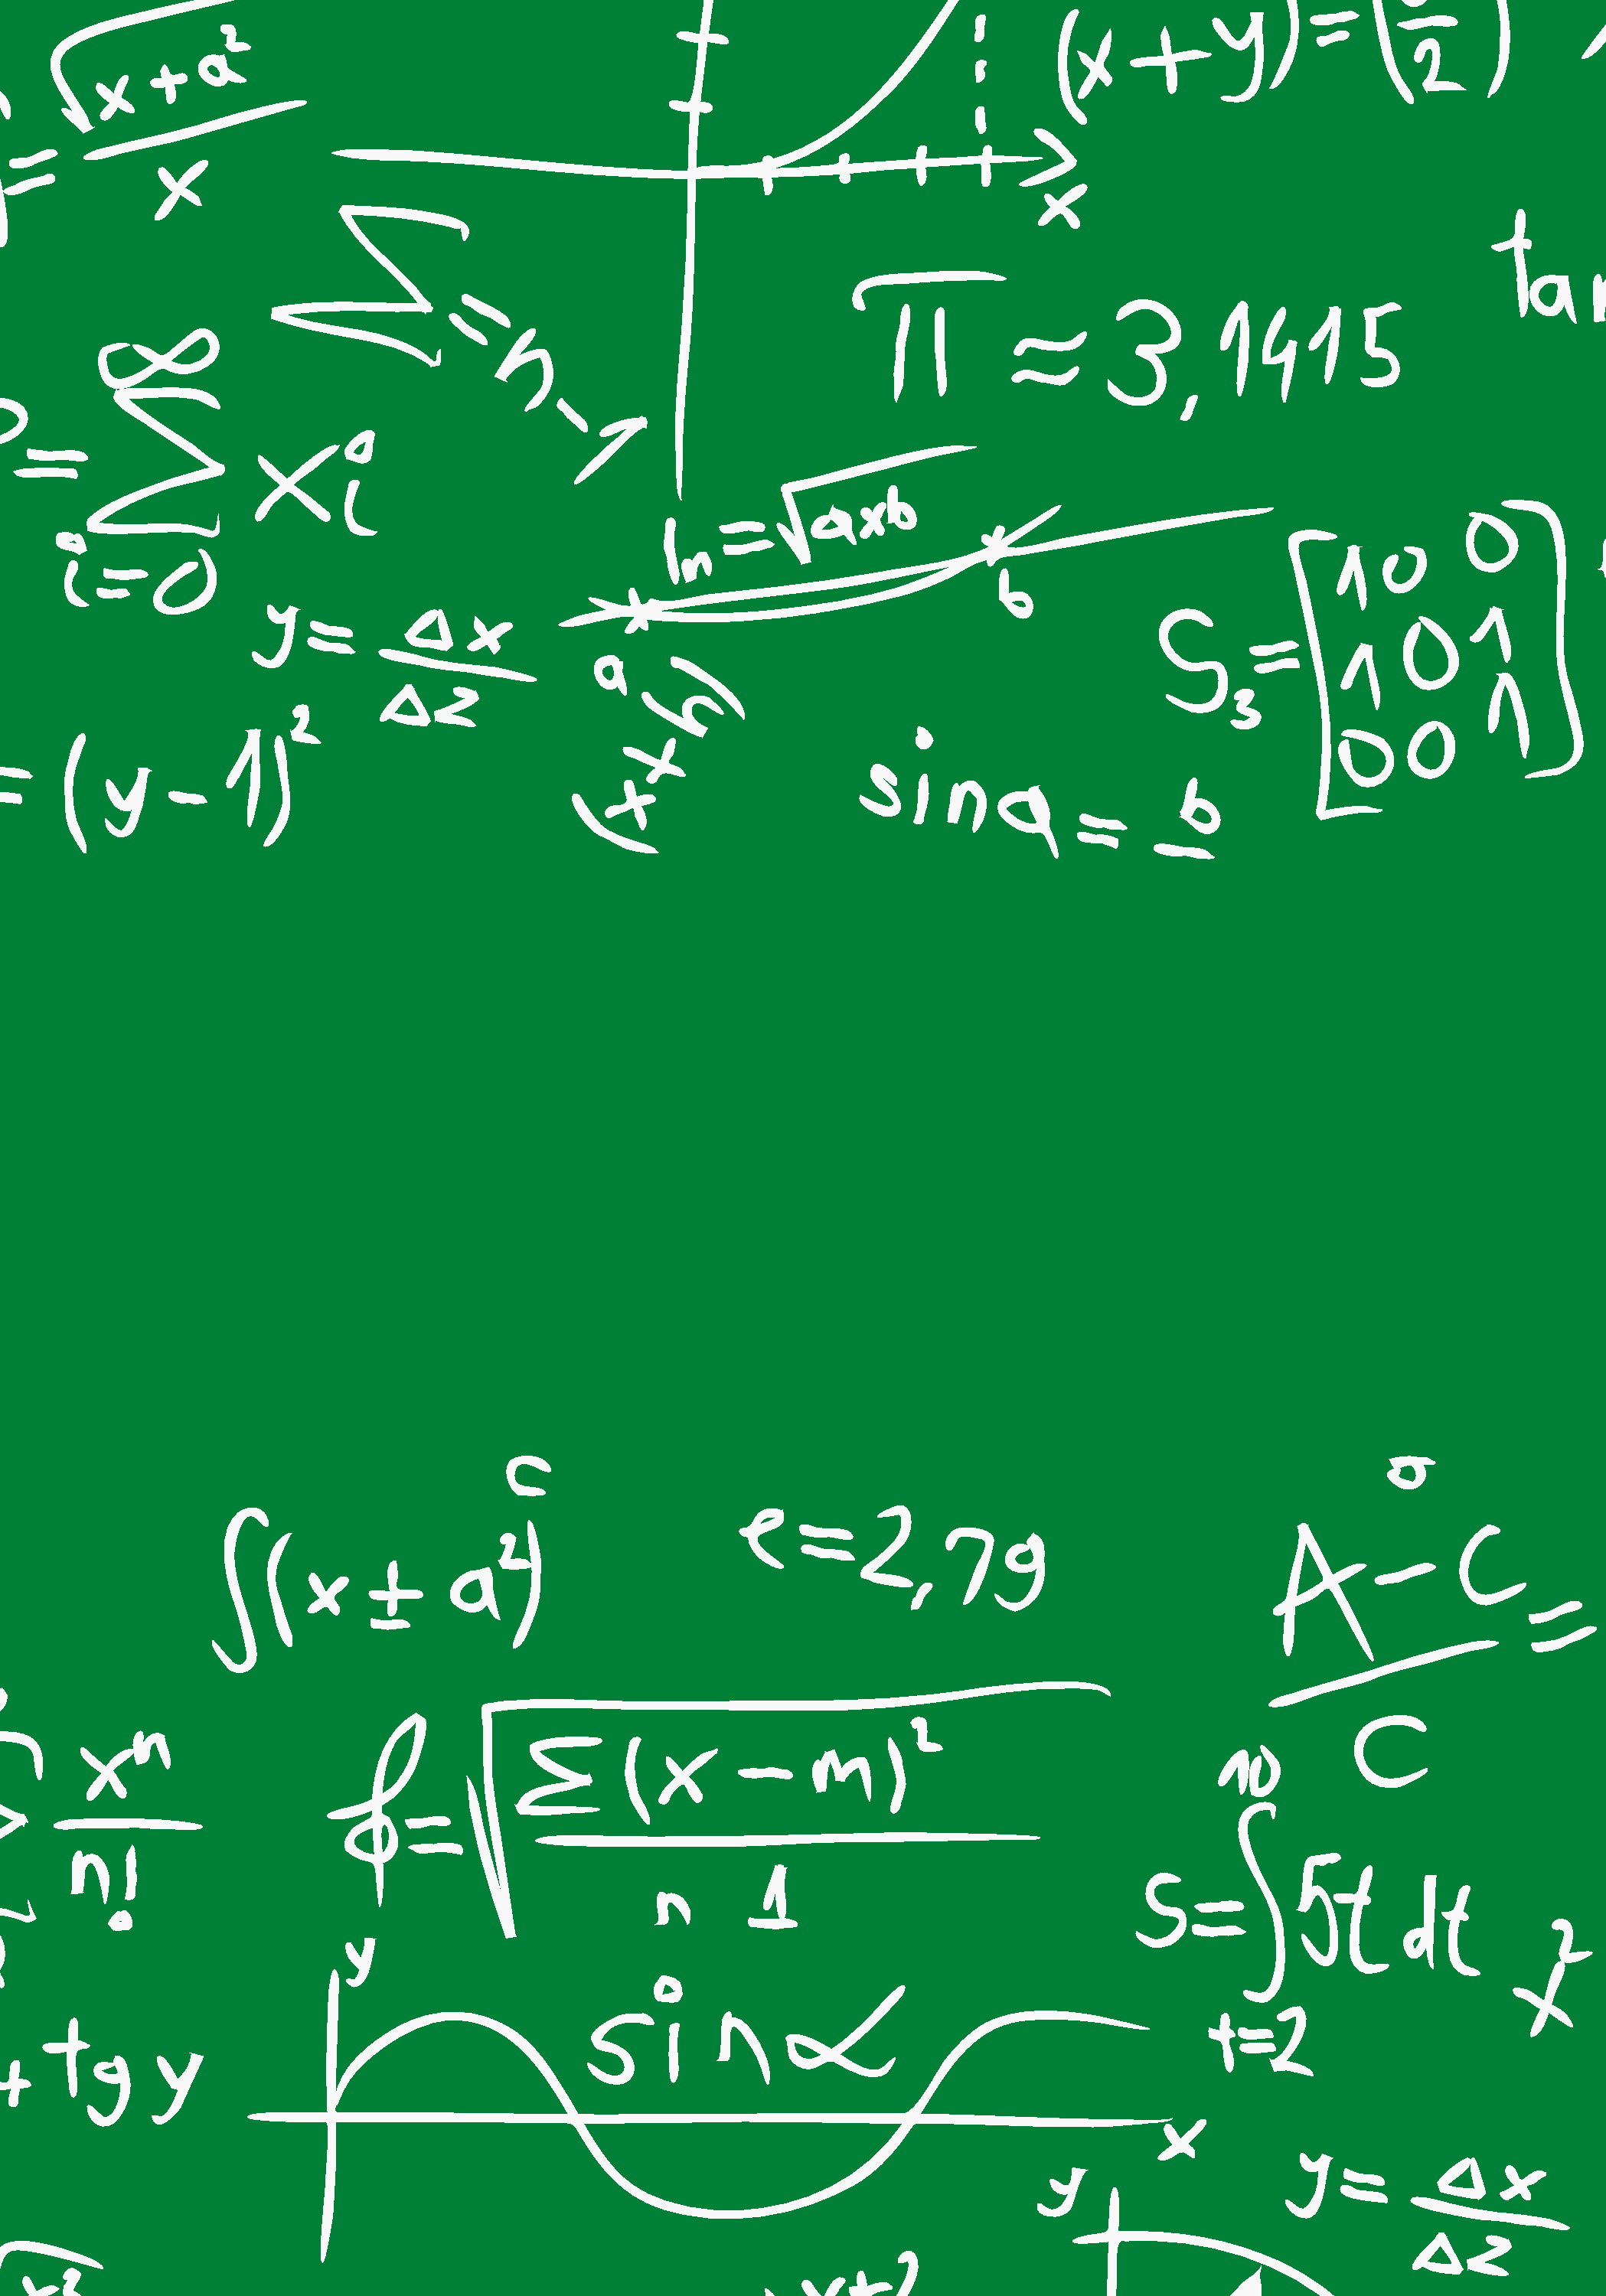
\includegraphics[width=\paperwidth]{Pictures/background.pdf}};
\draw (current page.center) node [fill=blue!30!white,fill opacity=0.6,text opacity=1,inner sep=1cm]{\Huge\centering\bfseries\sffamily\parbox[c][][t]{\paperwidth}{\centering Cálculo 3\\[15pt] % Book title
{\Large Notas de clases}\\[20pt] % Subtitle
{\huge Rudik Roberto Rompich}}}; % Author name
\end{tikzpicture}
\vfill
\endgroup

%----------------------------------------------------------------------------------------
%	COPYRIGHT PAGE
%----------------------------------------------------------------------------------------

\newpage
~\vfill
\thispagestyle{empty}

\noindent Copyright \copyright\ 2020 Rudik Rompich\\ % Copyright notice

\noindent \textsc{Published by Rudiks}\\ % Publisher

\noindent \textsc{rudiks.com}\\ % URL

\noindent Licensed under the Creative Commons Attribution-NonCommercial 3.0 Unported License (the ``License''). You may not use this file except in compliance with the License. You may obtain a copy of the License at \url{http://creativecommons.org/licenses/by-nc/3.0}. Unless required by applicable law or agreed to in writing, software distributed under the License is distributed on an \textsc{``as is'' basis, without warranties or conditions of any kind}, either express or implied. See the License for the specific language governing permissions and limitations under the License.\\ % License information, replace this with your own license (if any)

\noindent \textit{First printing, October 2020} % Printing/edition date

%----------------------------------------------------------------------------------------
%	TABLE OF CONTENTS
%----------------------------------------------------------------------------------------

%\usechapterimagefalse % If you don't want to include a chapter image, use this to toggle images off - it can be enabled later with \usechapterimagetrue

\chapterimage{Pictures/0001} % Table of contents heading image

\pagestyle{empty} % Disable headers and footers for the following pages

\tableofcontents % Print the table of contents itself

\cleardoublepage % Forces the first chapter to start on an odd page so it's on the right side of the book

\pagestyle{fancy} % Enable headers and footers again

%----------------------------------------------------------------------------------------
%	PART
%----------------------------------------------------------------------------------------

\part{Contenido Parcial 3}

%----------------------------------------------------------------------------------------
%	CHAPTER 1
%----------------------------------------------------------------------------------------

\chapterimage{Pictures/0001} % Chapter heading image

\chapter{Cálculo vectorial}


\section{28 de septiembre de 2020}
\subsection{Cálculo diferencial en varias variables - Funciones vectoriales}




\tikzset{every picture/.style={line width=0.75pt}} %set default line width to 0.75pt        

\begin{tikzpicture}[x=0.75pt,y=0.75pt,yscale=-1,xscale=1]
%uncomment if require: \path (0,310); %set diagram left start at 0, and has height of 310

%Shape: Axis 2D [id:dp34825501509521994] 
\draw  (23,212.3) -- (268.5,212.3)(47.55,44) -- (47.55,231) (261.5,207.3) -- (268.5,212.3) -- (261.5,217.3) (42.55,51) -- (47.55,44) -- (52.55,51)  ;
%Straight Lines [id:da7120917074211834] 
\draw    (47.55,212.3) -- (137.27,96.58) ;
\draw [shift={(138.5,95)}, rotate = 487.79] [color={rgb, 255:red, 0; green, 0; blue, 0 }  ][line width=0.75]    (10.93,-3.29) .. controls (6.95,-1.4) and (3.31,-0.3) .. (0,0) .. controls (3.31,0.3) and (6.95,1.4) .. (10.93,3.29)   ;
%Curve Lines [id:da9112376831548035] 
\draw    (18.5,137) .. controls (160.5,34) and (172.5,135) .. (210.5,113) ;
%Shape: Axis 2D [id:dp7523057169401708] 
\draw  (379,175.1) -- (547.5,175.1)(395.85,32) -- (395.85,191) (540.5,170.1) -- (547.5,175.1) -- (540.5,180.1) (390.85,39) -- (395.85,32) -- (400.85,39)  ;
%Straight Lines [id:da25097728151684107] 
\draw    (395.85,175.1) -- (313.84,265.52) ;
\draw [shift={(312.5,267)}, rotate = 312.21000000000004] [color={rgb, 255:red, 0; green, 0; blue, 0 }  ][line width=0.75]    (10.93,-3.29) .. controls (6.95,-1.4) and (3.31,-0.3) .. (0,0) .. controls (3.31,0.3) and (6.95,1.4) .. (10.93,3.29)   ;
%Curve Lines [id:da48745085294216717] 
\draw    (417,244) .. controls (505.5,158) and (482.5,55) .. (424.5,118) ;
%Curve Lines [id:da11758926162301764] 
\draw    (562.5,34) .. controls (595.5,39) and (427.5,217) .. (424.5,118) ;

% Text Node
\draw (138,57) node [anchor=north west][inner sep=0.75pt]    {$( x( t_{0}) ,y( t_{o}))$};
% Text Node
\draw (122,142) node [anchor=north west][inner sep=0.75pt]    {$r( t_{o})$};
% Text Node
\draw (405,61) node [anchor=north west][inner sep=0.75pt]    {$x( t_{o}) ,y( t_{o}) ,z( t_{o}))$};
% Text Node
\draw (483,134) node [anchor=north west][inner sep=0.75pt]    {$r( t_{o})$};


\end{tikzpicture}

\begin{definition}
\begin{align}
    \mi{x=f(t)&y=g(t)} a\leq t\leq b\\
    \mi{r(t)=\bv{f(t),g(t)}=f(t)\hat{i}+y(t)\hat{j}}\\
    \mi{r_o=\bv{x_o,x_o,z_o}&r_1=\bv{x_1,y_1,z_1}}\\
    \mi{t=(1-t)r_o+tr_1}
\end{align}
\end{definition}

\begin{exercise}
\begin{align}
    \intertext{¿Función vectorial? Para recta que va $P_o(3,2,-1)$ al punto $P_1(1,4,5)$}
    \mi{r(t)=(1-t)\bv{3,2,-1}+t\bv{1,4,5}}\\
    \mi{r(t)=\bv{3-2t,2+2t,-1+6t}}
\end{align}
\end{exercise}
%---
\begin{align}
    \mi{\vf{4\cos t}{+t}{+2\sin t}} &\text{c. helicoloides}
\end{align}
%---

\begin{align}
    \mi{\vf{t\cos t}{+t\sin t}{+t}}
\end{align}
%---
\begin{align}
    \mi{\vf{t^2}{+t^4}{+t^6}}
    \intertext{$x,y; y=x^3$ y $x,z; z=x^3$}
\end{align}

\subsection{Campos vectoriales}
\begin{definition}
\begin{align}
    \intertext{Sobre $\mathbf{R}^2$ una función $F$ que asigna a cada punto $(x,y)$ en $D$ (conjunto en $\mathbf{R}^2$) un vector bidimensional.}
    \mi{F(x,y)=\vfd{P(x,y)}{+Q(x,y)}}\\
    \mi{\bv{P(x,y),Q(x,y)}}\\
    \mi{F=P_i+Q_j}
    \intertext{También es posible expresarlas:}
    \mi{F(x,y,z)=\vf{P}{+Q}{+R}}
\end{align}
\end{definition}
%---
\begin{example}
\begin{align}
    \mi{F(x,y)=\vfd{-y}{+x}}\\
    \mi{||F||=C}\\
    \mi{\sqrt{y^2 +x^2}=C}
    \mi{x^2 +y^2 = C^2}\\
    \mi{(1,0)\mapsto\vfd{-(0)}{+(1)}=j}\\
    \mi{(0,1)\mapsto\vfd{-(1)}{+0}=-i}\\
    \mi{(1.5,1.5)\mapsto \vfd{-1.5}{+1.5}}
\end{align}
\end{example}
%---- 
\begin{example}
\begin{align}
    \mi{F(x,y)=\vfd{2x}{+y}}\\
    \mi{||F||=C}\\
    \mi{\sqrt{(2x)^2 +y^2}=C}\\
    \mi{4x^2 +y^2 =C^2 }& \text{elipse}\\
    \mi{(0.5,0)\implies 1i}\\
    \mi{(0,1)\implies 1j}\\
    \mi{(0.25,0.25)\implies \vfd{0.5}{+0.25}}\\
    \mi{(-2,-2)\implies \vfd{-4}{-2}}
\end{align}
\end{example}

%---- 
\begin{example}
\begin{align}
    \mi{F(x,y,z)=\vf{1}{-1}{0}}\\
    \mi{||F||=C}\\
    \mi{\sqrt{(1)^2 +(1)^2 +(0)^2}=\sqrt{2}}
\end{align}
\end{example}

\subsection{Gradiente}
\begin{definition}
\begin{align}
    \mi{f(x,y)=x^2 y+3xy^3}\\
    \mi{\nabla f(x,y)=\vfd{f_x(x,y)}{+f_y(x,y)})}\\
    \mi{\nabla f(x,y)=\vfd{(2xy+3y^3)}{+(x^2 +9xy^2)}}\\
    \intertext{Si $z=f(x,y)$}
\end{align}
\end{definition}

\begin{exercise}
\begin{align}
    \mi{f(x,y,z)=\sqrt{x^2+y^2+z^2}}\\
    \mi{\nabla(x,y,z)=\vf{\frac{x}{\sqrt{x^2 +y^2+z^2}}}{\frac{y}{\sqrt{x^2 +y^2+z^2}}}{\frac{z}{\sqrt{x^2 +y^2+z^2}}}}\\
\end{align}
\end{exercise}

\begin{exercise}
\begin{align}
    \intertext{Una partícula se mueve en un campo de velocidad $V(x,y)= \bv{x^2,x+y^2}$. Si su posición es (2,1) en un tiempo t=3, estime su posición en t=3.01}
    \mi{t=3\mapsto(2,1)}\\
    \mi{v(2,1)=\bv{2^2,2+1^2}=\bv{4,3}}\\
    \mi{t=3\mapsto3.01\implies0.001}\\
    \mi{0.01V(2,1)=0.01\bv{4,3}=\bv{0.04,0.03}}\\
    \mi{\text{Posición (2.04,1.03)}}
\end{align}
\end{exercise}
\subsection{Integral de Línea}
\begin{definition}
De $f$ a lo largo de $C$. 
\begin{align}
    \mi{\int_c f(x,y)ds = \lim_{n\mapsto\infty}}\suma{i=1}{n}{f(x_i^*,y_i^*)\Delta S}\\
    \intertext{$L=\ie{a}{b}{\sqrt{(\frac{dx}{dt})^2+(\frac{dy}{dt})^2}}{S}$}
    \mi{\int_c f(x,y)dS=\ie{a}{b}{f(x(t),y(t))*\sqrt{(\frac{dx}{dt})^2+(\frac{dy}{dt})^2}}{S}}
\end{align}
\end{definition}

\begin{exercise}
\begin{align}
    \mi{\ie{c}{}{(x^2-y+3z)}{S}}\\
    \intertext{x = t, y = 2t, z = t. En donde $0\leq t \leq$ }
    \intertext{x'=1,y=2,z=1.}
    \mi{\sqrt{(1)^2+(2)^2+(1)^2}=\sqrt{6}}\\
    \mi{\ie{c}{}{(x^2-y+3z)}{S}= \ie{0}{1}{(t^2 -2t +3t)\sqrt{6}}{t}}\\
    \mi{\sqrt{6}\ie{0}{1}{(t^2 +t)}{t}}\\
    \mi{\sqrt{6}[\frac{t^3}{3}+\frac{t^2}{2}]_0^1}\\
    \mi{=\frac{5\sqrt{6}}{6}}
\end{align}
\end{exercise}

\begin{exercise}
\begin{align}
    \mi{\ie{c}{}{(x+2)}{s}}
    \intertext{donde C es}
    \mi{r(t)=\vf{t}{+\frac{4t^{3/2}}{3}}{+\frac{t^2}{2}}}&0\leq t\leq 2\\
    \mi{||r'(t)||=\sqrt{(1)^2 +(2t^{1/2})^2+(t)^2}=\sqrt{1+4t+t^2}}\\
    \mi{\ie{c}{}{(x+2)}{s}=\ie{0}{2}{(t+2)\sqrt{1+4t+t^2}}{t}}\\
    \mi{=15.29}&x=t,y=\frac{4}{t^{2/2}},z=\frac{t^2}{2}
\end{align}
\end{exercise}



\section{29 de septiembre de 2020}

\begin{exercise}
¿Masa de un resorte?
\begin{align}
    \mi{r(t)=\frac{1}{\sqrt{2}}\vfd{\cos t}{\sin t}{t}}& 0\leq t \leq 6\pi\\ 
    \mi{||r'(t)||=\frac{1}{\sqrt{2}}\sqrt{(-sent)^2+(cost)^2 +(1)^2}=1}\\
    \mi{\frac{1}{\sqrt{2}}\sqrt{2}= \frac{\sqrt{2}}{\sqrt{2}}}\\
    \mi{\ie{c}{}{(1+z)}{S}=\ie{0}{6\pi}{(1+\frac{t}{\sqrt{2}})(1)}{t}}\\
    \mi{[t +\frac{t^2}{2\sqrt{2}}]_0^{6\pi}= 6\pi(1+\frac{3\pi}{\sqrt{2}})=144.47}
\end{align}
\end{exercise}

\begin{exercise}

\begin{align}
    \mi{\ie{c}{}{f(x,y)}{x}=\ie{a}{b}{f(x(t),y(t))x'(t)}{t}}\\
    \mi{\ie{c}{}{xy^2}{x}}& x=4cost,y=4sent & 0\leq t\leq \frac{\pi}{2}&\\
    \mi{\ie{c}{}{xy^2}{x}=\ie{0}{\pi/2}{(4cost)(16\sin^2 t)(-4sent)}{t}}\\
    \mi{-256\ie{0}{\pi/2}{\sin^2t*cost}{t}=-256[\frac{\sin^4 t}{4}]_0^{\pi/2}=-64}
\end{align}
\end{exercise}

\begin{exercise}
\begin{align}
    \mi{\ie{c}{}{f(x,y)}{x}=\ie{a}{b}{f(x(t),y(t))y'(t)}{t}}\\
    \mi{\ie{c}{}{xy^2}{x} & x=4\cos t,y=4\sin t & 0\leq t\leq \frac{\pi}{2}}\\
    \mi{\ie{c}{}{xy^2}{x}=\ie{0}{\pi/2}{(4cost)(16\sin^2 t)(4cost)}{t}}\\
    \mi{256\ie{0}{\pi/2}{\sin^2t*cost}{t}=256\ie{0}{\pi/2}{\frac{\sin^2 2t}{4}}{t}\\
    \mi{=64\ie{0}{\pi/2}{\frac{1}{2}(1-cos(4t)}{t}}}\\
    \mi{=16\pi}
\end{align}
\end{exercise}

\begin{exercise}
\begin{align}
    \mi{\ie{c}{}{f(x,y)}{x}=\ie{a}{b}{f(x(t),y(t))||f||}{t}}\\
    \mi{\ie{c}{}{xy^2}{x} & x=4\cos t,y=4\sin t & 0\leq t\leq \frac{\pi}{2}}\\
    \mi{\ie{c}{}{xy^2}{x}=\ie{0}{\pi/2}{(4cost)(16\sin^2 t)(\sqrt{16(\cos^2 t+\sin^2 t)})}{t}}\\
    \mi{256/3}
\end{align}
\end{exercise}

\begin{exercise}
\begin{align}
    \mi{\ie{c}{}{xy}{x}+x^2 dy & c:y=x^3 & -1\leq x \leq 2}\\
    \mi{\ie{-1}{2}{x(x^3)}{x}+x^2 (3x^2 dx)}& dy=3x^2 dx\\
    \mi{\ie{-1}{2}{4x^4}{x}=\frac{4x^5}{5}|_{-1}^2=\frac{132}{5}}
\end{align}
\end{exercise}

\begin{exercise}

\begin{align}
    \mi{\ie{c}{}{y^2}{x}-x^2dy}
    \intertext{$\int_c =\int_{c_1} + \int_{c_2} + \int_{c_3}$}
    \mi{\ie{c_1}{}{y^2}{x}-x^2dy& y=0,dy=0dx}\\
    \mi{= \ie{0}{2}{(0)^2}{x}-x^2 (0dx) =0}\\
    \mi{\ie{c_2}{}{y^2}{x}-x^2 dy = \ie{0}{4}{y^2 (0}{y)-4dy}} & x=2,dx=0dy\\
    \mi{[-4y]_0^4 =-16}\\
    \mi{\ie{c_3}{}{y^2}{x}-x^2 dy = \ie{2}{0}{x^4}{x}-x^2(2xdx)}\\
    \mi{\ie{2}{0}{(x^4 -2x^3)}{x}=[(\frac{x^5}{5}-\frac{x^4}{2})]_2^0 =8/5}\\
    \mi{\ie{c}{}{y^2}{x}-x^2dy= 0+(-16)+8/5 =-72/5}
\end{align}
\end{exercise}

\subsection{Definición de trabajo}
\begin{definition}
\begin{align}
    \mi{W=\ie{a}{b}{f(x)}{x}}\\
    \mi{\text{Fuerza constante. }} & F\mapsto W=F\cdot D & D=\Vec{PQ}\\
    \mi{\ie{c}{}{F\cdot}{r}=\ie{a}{b}{F(r(t))\cdot r'(t)}{t}}
\end{align}
\end{definition}

\ej{
\mi{F(x,y,z)=\vfd{-\frac{1}{2}x}{-\frac{1}{2}}{+\frac{1}{4}}}\\
\mi{r(t)=\vf{cost}{+sent}{+t}}\\
\mi{(1,0,0)\mapsto (-1,0,3\pi)}&x=cost,y=sent,z=t\\
\mi{F(x(t),y(t),z(t))= \vfd{-\frac{cost}{2}}{-\frac{sent}{2}}{\frac{1}{4}}}\\
\mi{r'(t)=\vf{-sent}{+cost}{+1}}\\
\mi{\ie{c}{}{F\cdot}{r}=\ie{0}{3\pi}{(\vfd{-\frac{cost}{2}}{-\frac{sent}{+2}}{+\frac{1}{4}})\cdot(\vf{-sent}{+cost}{+1})}{t}}\\
\mi{\ie{0}{3\pi}{(\frac{costsint}{2})-\frac{costsent}{2}+\frac{1}{4}}{t}}\\
\mi{\ie{0}{3\pi}{\frac{1}{4}}{t}=[\frac{1}{4}t]_0^{3\pi}=\frac{3\pi}{4}}
}

\ej{
\intertext{$F(x,y)=\vfd{y}{+x}$ a lo largo de $y=ln(x)$ desde (1,0) hasta (e,1). ¿Cuál es el w?}
\mi{w=\ie{c}{}{F\cdot}{r}}&r(t)=\vfd{x}{+lnx}\\
\intertext{Parametrización de x}
\mi{F= \vfd{lnx}{+x}}\\
\mi{dr=(\vfd{1}{+\frac{1}{x}})dx}\\
\mi{w= \ie{1}{e}{lnx}{x}+\ie{1}{e}{1}{dx}}
\mi{xln(x) -\ie{1}{e}{1}{x}+\ie{1}{e}{1}{x}=[xln(x)]_1^e =e}
}

\ej{
\intertext{¿w? $F(x,y) =\vfd{a}{b}$ alrededor de $x^2+y^2=9\longleftarrow r=\vfd{3\cos t}{+3\sin t}$ en donde $0\leq t \leq 2\pi$}
\intertext{$dr= \vfd{-3\sin t}{+\cos t}$}
\mi{w=\ie{0}{2\pi}{(-3asent+3bcost)}{t}=[3acost +3bsent]_0^{2\pi}=0}
}
\ej{
}
\section{5 de octubre de 2020}

\dn{
\text{Campo vectorial conservativo}\\
\intertext{$F$ si, existe una función f tal que $\nabla f = F$ .$f\mapsto$ función de potencial para $F$.}
}

\ej{
\mi{F(x,y)=\vfd{y}{+x}}& \nabla f=F\\
\mi{\nabla f =\vfd{\derivada{f}{x}}{+\derivada{f}{y}}= \vfd{y}{+x}}&\text{F es conservativo}\\
\mi{f(x,y)=xy}
}

\ej {
\mi{F(x,y)=\vfd{cosx}{+(a+seny)}}\\
\mi{f(x,y)=senx+y+cosy}& \nabla f=F\\
\mi{\derivada{f}{x}=cosx& \derivada{d}{y}=(1-seny)}
}

\ej{
\mi{F(x,y,z)=\vf{y^2 z^3}{2xyz^3}{3xy^2 z^2}}\\
\mi{f(x,y,z)=xy^2 z^3}&\nabla f=F\\
\mi{\derivada{f}{x}= y^2 z^3 }
}

\begin{theorem}
\begin{align}
    \intertext{Teorema fundamental de las integrales de línea}
    \mi{\ie{a}{b}{F'(x)}{x}= F(b)-F(a)}& \text{ antiderivada}\\
    \intertext{Función vectorial $r(t)$ en donde $a\leq t \leq b$ tal que $f$ es derivable $\nabla f$ es continuo}\\
    \mi{\ie{c}{}{\nabla f\cdot}{r}=f(r(b)-f(r(a))}\\
\end{align}
\end{theorem}

\ej{
\mi{\vf{yz}{xz}{xy}}& \text{donde: } f(x,y,z)=xyz\\
\intertext{A(-1,3,) hasta el punto B(1,6,-4)}\\
\mi{w= \ie{c}{}{F\cdot}{r}= \ie{A}{B}{\nabla f\cdot}{r}=f(B)-f(A)}\\
\mi{xyz|_(1,6,-4)- xyz|_(-1,3,9)}\\
\mi{(1)(-4)(6)-(-1)(3)(9)=3}
}

\begin{theorem}
\begin{align}
    \intertext{Teorema $\ie{c}{}{F\cdot}{r}$ es independiente de su trayectoria en $D$ ssi $\ie{c}{}{F\cdot}{r}$ es igual para toda trayectoria cerrada.}
\end{align}
\end{theorem}

\ej{
\mi{F(x,y)=\vfd{P(x,y)}{+Q(x,y)}}\\
\mi{\derivada{P}{y}=\derivada{Q}{x}}
}

\ej{
\mi{F(x,y)= \vfd{-ye^{-xy}}{-xe^{-xy}}}&P=-ye^{-xy}&Q=-xe^{-xu¡y}\\
\mi{\derivada{P}{y}=xye^{-xy}-e^{-xy}}\\
\mi{\derivada{Q}{x}=xye^{-xy}-e^{-xy}}\\
\mi{\derivada{P}{y}=\derivada{Q}{x}}\\
\text{F es conservativo.}
}

\ej{
\mi{F(x,y)=\vfd{(x^2 -2y^3)}{(x+5y)}}\\
\mi{P=x^2 -2y^3 & Q=x+5y}\\
\mi{\derivada{P}{y}=-6y^2 \neq \derivada{Q}{x}=1}
}
\dn{
\mi{F=\vf{P(x,y,z)}{+Q(x,y,z)}{+R(x,y,z)}}\\
\mi{\derivada{P}{y}=\derivada{Q}{x}&\derivada{P}{z}=\derivada{R}{x} &\derivada{Q}{z}=\derivada{R}{y}}\\
}

\ej{
\mi{F=\vf{(e^x cosy +yz)}{+(xz-e^x seny)}{(xy+z)}}\\
\mi{\derivada{P}{y}=\derivada{Q}{x}=-e^x seny+z}\\
\mi{\derivada{P}{z}=\derivada{R}{x}=y}\\
\mi{\derivada{Q}{z}=\derivada{R}{y}=x}\\
\text{F sí es conservativo}.\\
\mi{\derivada{f}{x}=(e^x cosy +yz) &\derivada{f}{y}=xz-e^x seny & \derivada{f}{z}=xy+z }\\
\mi{f(x,y,z) =e^x cosy +xyz +g(y,z)}\\
\intertext{$\derivada{g}{y}=xz-xz-e^x seny +e^x seny=0$}
\mi{\derivada{f}{y}=-e^x seny +xz+\derivada{g}{y}= xz-e^x seny}\\
\mi{f(x,y,z)=e^x cosy+xyz +h(z)}\\
\mi{\derivada{f}{z}=xy+\derivada{h}{z}=xy+z}
\mi{\derivada{h}{z}=z}\\
\mi{h(z)=\frac{z^2}{2}+c}\\
\mi{f(x,y,z)=e^x cosy +xyz +\frac{z^2}{2}+c}
}

\ej{
\mi{F=\vf{-\frac{y}{x^2 +y^2}}{+\frac{x}{x^2 +y^2}}{0}}\\
\mi{\derivada{P}{y}=\derivada{Q}{x}=\frac{-x^2+y^2}{(x^2+y^2)^2}}\\
\mi{\derivada{P}{z}=\derivada{R}{x}=0}\\
\mi{\derivada{Q}{z}=\derivada{R}{y}=0}\\
\text{F no es conservativo}
}

\ej{
\mi{r(t)=\vfd{cost}{+sent}}& 0\leq t \leq 2\pi \\
\mi{F=\vfd{-\frac{sent}{(\sin^2)+(\cos^2 t)}}{+\frac{\cos t}{(\sin^2)+(\cos^2 t)}}}\\
\mi{= \vfd{-sent}{+cost}}\\
\mi{dr=\vfd{(-sent}{+cost}}\\
\mi{\ie{c}{}{F\cdot}{dr}=\ie{c}{}{F\cdot\frac{dr}{dt}}{t}=\ie{0}{2\pi}{(sen^2 t +cos^2 t)}{t}=2\pi}
}
\ej{
\mi{\ie{c}{}{(y+yz)}{x}+(x+3z^2+xz)dy+(9yz^2 +xy-1)dz)}\\
\intertext{Demostrar que es independiente de la trayectoria (1,1,1) y (2,1,4)}
\mi{\derivada{P}{y}=\derivada{Q}{z}=1+z}\\
\mi{\derivada{P}{z}=\derivada{R}{x}=y}\\
\mi{\derivada{Q}{z}=\derivada{R}{y}=9z^2 +x}\\
\mi{\ie{(1,1,1)}{(2,1,4)}{F\cdot}{r}}\\
\mi{f=xy+xyz+g(y,z)}\\
\mi{\derivada{f}{y}=x+xz+\derivada{g}{y}= x+3z^2 +xz}& \derivada{g}{y}=3z^2\\
\mi{g(y}=3yz^3 +h(z)\\
\mi{f=xy+xyz+3yz^3 +h(z)}\\
\mi{\derivada{f}{z}=xy+9yz^2+\derivada{h}{z}=9yz^2 +xy-1}& h(z)=-z+c\\
\mi{f=xy+xyz+3yz^3+(-z)}\\
\mi{\ie{(1,1,1)}{(2,1,3)}{F\cdot}{r}=[xy+xyz+3yz^3 -z]_{(1,1,1)}^{(2,1,4)}=198-40=194}
}



\section{13 de octubre de 2020}

\ej{
\mi{\ie{(0,0,0)}{(2,3,-6)}{2x}{x}+3ydy+2zdz}\\
\mi{ \ie{(0,0,0,0)}{(2,3,6)}{F\cdot}{r}}\\
\mi{F(x,y,z)=\vf{2x}{+2y}{+2z}}& \derivada{P}{y}=0=\derivada{Q}{x}\\
\mi{\derivada{Q}{z}=0=\derivada{R}{y}}& \derivada{P}{z}=0=\derivada{R}{x}&F=\nabla f\\
\mi{\derivada{f}{x}=2x} & f(x,y,z)=x^2 +g(y,z)\\
\mi{\derivada{f}{y} =\derivada{q}{y}=2y \mapsto g(y)=y^2 +h(z)}\\
\mi{\derivada{f}{z}=\derivada{h}{z}=2z \mapsto h(z)=z^2 }\\
\mi{\ie{(0,0,0)}{(2,3,-6)}{2x}{x}+3ydy+2zdz}\\
\mi{= [(x^2 +y^2 +z^2)]_{0,0,0}^{2,3,-6}=z^2 +3^2 +(-6)^2 =49}
}

\ej{
\mi{\ie{(1,0,0)}{(0,1,1)}{senycosx}{x}+cosysenxdy+dz}\\
\mi{\derivada{P}{y}=\derivada{Q}{x}=cosycosx}& \derivada{Q}{z}=\derivada{R}{y}=0 & \derivada{P}{z}=\derivada{R}{x}=0\\
\mi{\derivada{f}{x}=senycosx}& f(x,y,z)=senysenx+g(y,z)\\
\mi{\derivada{f}{y}=cosysenx +\derivada{g}{y}=cosysenx}& g(y)=h(z)\\
\mi{\derivada{f}{z}= \derivada{h}{z}=1}& h(z)=z & f(x,y,z)=senysenx +z\\
\mi{\ie{(1,0,0)}{(0,1,1)}{F\cdot}{r}=[senysenx+z]_{(1,0,0)}^{(0,1,1)}=1}
}

\ej{
\intertext{$F=\nabla(x^3 y^2)$ y C: trayectoria en plano xy que va desde (-1,1) a (1,1) y que consiste en los segmentos. (-1,1) a (0,0) y (0,0) a (1,1)}
\intertext{Evalúe $\ie{c}{}{F\cdot}{r}$ para los parámetros.}
\mi{F=\nabla(x^3 y^2)\implies F=\vfd{3x^2 y^2}{+2x^3 y}}\\
\mi{C_1:(-1,1)\implies(0,0)}\\
\mi{x= t-1 & y=-t+1 & 0\leq t \leq 1}\\
\mi{F=\vfd{3(t-1)^2(-t+1)^2}{2(t-1)^3 (-t+1)}}\\
\mi{r=\vfd{(t-1)}{(-t+1)}}\\
\mi{dr= \vfd{dt}{-dt}}\\
\mi{\ie{0}{1}{(3(t-1)^2 (-t+1)^2}{t}-2(t-1)^3 (-t+1)dt =1}\\
\mi{C_2: (0,0)\mapsto(1,1)}\\
\mi{ x=t & y=t & 0\leq t \leq 1}\\
\mi{F=\vfd{3t^4}{+2t^4}}\\
\mi{r=\vfd{t}{t} & dr= \vfd{dt}{dt}}\\
\mi{\ie{0}{1}{(3t^4 + 2t^4)}{t}=1}\\
\mi{\ie{c_1}{}{F\cdot}{r}+\ie{c_2}{}{F\cdot}{r}=1+1 =2}
\intertext{Use $f(x,y)=x^3 y^2$ como una función potencial para F. }\\
\mi{f(x,y)=x^3 y^2= \ie{(-1,1)}{(1,1)}{F\cdot}{r}= [x^3 y^2 ]_{(-1,1)}^{(1,1)}= 1-(-1) =2}
}
\section{12 de octubre de 2020}
\subsection{Teorema de Green}

\begin{remark}
\textbf{Orientación positiva: } Sentida antihorario.\\ 
\textbf{Orientación negativa: } Sentida horario. 
\end{remark}

\ej{
\mi{\oint_{C} (x^2-y^2)dx +(2y-x)dy}\\
\mi{ c:y=x^2, y=x^3}\\
\mi{P=x^2-y^2}\\
\mi{Q=2y-x}\\
\mi{\derivada{Q}{x}=-1}& \derivada{P}{y}=-2y\\
\mi{\iint_{D}(-1-(-2y))dA=\int_{0}^{1}\int_{x^3}{x^2}(-1+y)dydx}\\
\mi{ \ie{0}{1}{[-y+y^2]_{x^3}^{x^2}}{x}=\ie{0}{1}{(-x^6+x^4 +x^3 -x^2)}{x}}\\
\mi{\frac{-x^7}{7}+\frac{x^5}{5}+\frac{x^4}{4}-\frac{x^3}{4}]_{0}^{1} = \frac{-11}{420}}
}

\ej{
\mi{\ieo{C}{}{(x^5+3y)}{x}+(2x-e^{y^2})dy} & c:(x-1)^2 +(y-5)^2 =4\\
\mi{P=x^5 +3y}& \derivada{P}{y}=3\\
\mi{Q=2x-e^{y^2}}& \derivada{Q}{x}=2\\
\mi{\iint_D (2-3)dA= -\iint_D 1dA} &A=\pi r^2 =\pi(2)^2 =4\pi\\
\mi{-\iint_P 1dA=-4\pi }
}
\ej{
\mi{F=\vfd{(-16y+sen(x^2)}{+(4e^{y}+3x^2)}}\\
\mi{w=\ieo{c}{}{F\cdot}{r}}\\
\mi{w=\ieo{c}{}{(-16y +sen(x^2))}{x}+(4e^y +3x^2)dy}\\
\mi{w=\iint_D (6x+16)dA= \ied{\pi/4}{3\pi/4}{0}{1}(6rcos\theta +16)rdrd\theta}\\
\mi{= \ied{\pi/4}{3\pi/4}{0}{1}(6r^2cos\theta +16r)drd\theta}\\
\mi{=\ie{\pi/4}{3\pi/4}{(2r^3 cos\theta +8r^2)]_0^1}{\theta}}\\
\mi{=\ie{\pi/4}{3\pi/4}{(2cos\theta+8)}{\theta}}
\mi{4\pi}
}

\dn{
\mi{\iint_D (\derivada{Q}{x}-\derivada{P}{y})dA}\\
\mi{\iint_{D_1} (\derivada{Q}{x}-\derivada{P}{y})dA +\iint_{D_2}(\derivada{Q}{x}-\derivada{P}{y})dA}\\
\mi{= \oint_{C_1} Pdx+Qdy + \oint_{C_2}Pdx+Qdy}\\
\mi{= \oint_{C} Pdx+Qdy}
}

\ej{
\mi{\oint_c \frac{1}{3}y^3 dx+(xy+xy^2)dy}\\
\intertext{c: es la frontera de la región en el primer cuadrante de $y=0,x=y^2,x=1-y^2$}
\mi{P=\frac{1}{3}y^3}& P_y=y^2\\
\mi{Q=xy+xy^2}& Q_x=y+y^2\\
\mi{\iint_D[(y+y^2)-y^2]dA= \ied{0}{\frac{1}{\sqrt{2}}}{y^2}{1-y^2}(y)dxdy}\\
\mi{\int_0^{1/\sqrt{2}}xy]_{y^2}^{1-y^2}=\ie{0}{1/\sqrt{2}}{(y-2y^3)}{y}=\frac{y^2}{2}-\frac{y^4}{2}]_{0}^{1/\sqrt{2}}=\frac{1}{8}}
}

\ej{
\mi{\oint_c e^{x^2}dx+2\tan^{-1} x dy}\\
\intertext{triángulo con vértices (0,0),(0,1),(-1,1)}
\mi{P=e^{x^2}}& Q=2\tan^{-1}x\\
\mi{P_y=0}& Q_x =\frac{2}{1+x^2}\\
\mi{\oint_c e^{x^2}dx+2\tan^{-1}xdy=\iint_D \frac{2}{1+x^2}dA}\\
\mi{\ied{-1}{0}{-x}{1}\frac{2}{1+x^2}dydx}\\
\mi{\int_{-1}^0 \frac{2y}{1+x^2}]_{-x}^1 dx=\ie{-1}{0}{(\frac{2}{1+x^2}+\frac{2x}{1+x^2})}{x}}\\
\mi{[2\tan^{-1}x+ln(1+x^2)]_{-1}^0 = \frac{\pi}{2}-ln(2)=0.87}
}
 \section{13 de octubre de 2020}
 
 \ej{
 \mi{\oint_c (4x^2-y^3)dx+(x^3 +y^2)dy}\\
 \intertext{La gráfica: $x^2+y^2=1$ y $x^2 +y^2 =4$}
 \mi{P_y=-3y^2} & Q_x =3x^2\\
 \mi{\iint_d (3x^3+3y^2)dA = \ied{0}{2\pi}{1}{2}3r^2 r drd\theta}\\
 \mi{\ie{0}{2\pi}{\frac{3r^4}{4}}{\theta}]_1^2}\\
 \mi{\ie{0}{2\pi}{\frac{45}{4}}{\theta} =\frac{45\pi}{2}}\\
 }
 %---- Me dio pereza xdxdxd, si alguien lee esto, que sepa que en este momento de la vida, realmente dudaba de mi mismo; aunque al final, creo que esta clase saldrá. 
 
 
 


\end{document}
